\section{Examples of the Morse complex} \label{section:morse_examples}

In this section we are going to provide some examples of the Morse complexes constructed in various manifolds these examples are meant to illustrate the properties of the Morse homology, as well as give some sense to how the theory is developed.

\subsection{The sphere}

\begin{exmpl}
Consider the 2 dimensional sphere embedded inside $\R^3$ and the height function $h(x,y,z) = z$ (restricted to $\con{S}^2$). As we saw in \ref{coro:reeb}, the spheres are the only compact manifolds without boundary that admit only two critical points, and the height function is the prime example of this.

\begin{figure}[h]
	\centering
	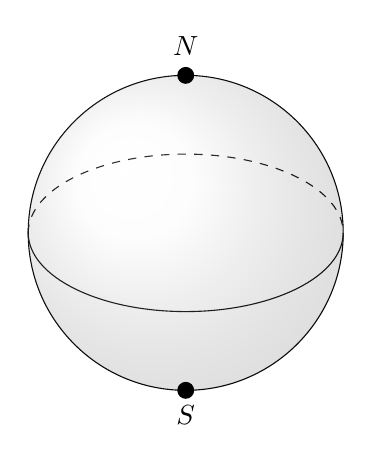
\begin{tikzpicture}
	\draw (-2,0) arc (180:360:2cm and 1cm);
	\draw[dashed] (-2,0) arc (180:0:2cm and 1cm);
	\draw (0,0) circle (2cm);
	\shade[ball color=gray!10!white,opacity=0.20] (0,0) circle (2cm);
	\draw [fill] (0,2) circle [radius=0.1cm]
	node [label={[above]$N$}] {};
	\draw [fill] (0,-2) circle [radius=0.1cm]
	node [label={[below,yshift=-0.2cm]$S$}] {};
\end{tikzpicture}
	\caption{The critical points of $h$ on $\con{S}^2$.}
	\label{figure:example1}
\end{figure}

In this case (see figure \ref{figure:example1}), the complex is easy to construct. The only critical points of $h$ are $S$ (of index 0) and $N$ of index 2, and the vector field $- \grad h$ (defined using the euclidean metric) satisfies the Smale condition, so we can use it to define the differential of the complex. However, we just commented that
\[C_k(\con{S}^2,h) = \left\{ \begin{array}{lc} \con{Z}_2 S & \text{if } k=0 \\ \con{Z}_2 N & \text{if } k=2 \\ 0 & \text{otherwise} \end{array} \right. ,\]
so $\partial_k = 0$ for all $k$. Therefore, the homology that results is the one that we might expect:
\[H_k(\con{S}^2,h) = \left\{ \begin{array}{lc} \con{Z}_2 & \text{if } k=0,2 \\ 0 & \text{otherwise} \end{array} \right. .\]
\end{exmpl}

\begin{exmpl} Let us think about a different function on the sphere. This function, $f$ is such that it induces the dynamics shown in Figure \ref{figure:example2}. In particular, it has the following critical points:
\begin{itemize}
	\item The local maxima $a_1,a_2$ and $a_3$, which are critical points of index $2$.
	\item The critical points $b_1$ and $b_2$ of index $1$.
	\item The absolute minimum $c$, of index $0$.
\end{itemize}

\begin{figure}[h]
	\centering
	\begin{tikzpicture}
	%Sphere
	\draw (-3,0) arc (180:360:3cm and 1.5cm);
	\draw[dashed] (-3,0) arc (180:0:3cm and 1.5cm);
	\draw (0,0) circle (3cm);
	\shade[ball color=gray!10!white,opacity=0.20] (0,0) circle (3cm);

	%Point a_1
	\draw [fill] (0,3) circle [radius=0.1cm]
	node [label={[above]$a_1$}] {};
	%Point a_2
	\draw [fill] (-2,-1.5) circle [radius=1mm]
	node [label={[below,xshift=3mm,yshift=-2mm]$a_2$}] {};
	%Point a_3
	\draw [fill=gray!90!white,draw=gray!90!white] (2,-1.5) circle [radius=1mm]
	node [label={[below,xshift=-3mm,yshift=-2mm]$a_3$}] {};
	%Point b_1
	\draw [fill] (-2,1.5) circle [radius=0.1cm]
	node [label={[above,xshift=-0.5mm,yshift=-0.6mm]$b_1$}] {};
	%Point b_2
	\draw [fill=gray!90!white,draw=gray!90!white] (2,1.5) circle [radius=0.1cm]
	node [label={[above,yshift=-0.6mm,xshift=1mm]$b_2$}] {};
	%Point c
	\draw [fill] (0,-3) circle [radius=0.1cm]
	node [label={[below,yshift=-0.2cm]$c$}] {};

	%Trajectory from a_1 to b_1
	\draw[-{Latex[length=2mm]}] (0,3) to [out=190,in=40] (-1.3,2.4);
	\draw[] (-1.2,2.5) to [out=220,in=60] (-2,1.5);
	\draw (-1.1,2.4) node [label={[below]$\lambda_1$}] {};

	%Trajectory from a_1 to b_2
	\draw[-{Latex[length=2mm]},dashed] (0,3) to [out=350,in=140] (1.3,2.4);
	\draw[dashed] (1.2,2.5) to [out=320,in=120] (1.95,1.6);
	\draw (1.1,2.4) node [label={[below]$\lambda_2$}] {};

	%Trajectory from a_2 to b_1
	\draw[-{Latex[length=2mm]}] (-2,-1.5) to [out=120,in=275] (-2.4,-0.4);
	\draw[] (-2.4,-0.45) to [out=95,in=240] (-2,1.5);
	\draw (-2.4,-0.5) node [label={[above,xshift=2.5mm]$\lambda_3$}] {};

	%Trajectory from a_3 to b_2
	\draw[-{Latex[length=2mm]},dashed] (2,-1.5) to [out=60,in=265] (2.4,-0.4);
	\draw[dashed] (2.4,-0.45) to [out=85,in=300] (2.05,1.4);
	\draw (2.4,-0.5) node [label={[above,xshift=-2mm]$\lambda_4$}] {};

	%Trajectory from b_1 to c
	\draw[-{Latex[length=2mm]}] (-2,1.5) to [out=330,in=110] (-0.49,-0.51);
	\draw[] (-0.5,-0.5) to [out=290,in=100] (0,-3);
	\draw (-0.5,-0.5) node [label={[above,xshift=-3.7mm]$\mu_1$}] {};

	%Trajectory from b_2 to c
	\draw[-{Latex[length=2mm]},dashed] (2,1.5) to [out=210,in=70] (0.5,-0.5);
	\draw[dashed] (0.5,-0.5) to [out=250,in=80] (0,-3);
	\draw (0.5,-0.5) node [label={[above,xshift=4mm]$\mu_3$}] {};

	%Trajectory from b_1 to c (behind)
	\draw[] (-2,1.5) to [out=150,in=80.41] (-2.96,0.5);
	\draw[-{Latex[length=2mm]},dashed] (-2.96,0.5) to [out=260.41,in=150] (-1.1,-2.6);
	\draw[dashed] (-1.1,-2.6) to [out=330,in=165] (0,-3);
	\draw (-1.1,-2.6) node [label={[above,xshift=2mm,yshift=-1.5mm]$\mu_2$}] {};

	%Trajectory from b_2 to c (in front)
	\draw[dashed] (2,1.5) to [out=30,in=99.59] (2.96,0.5);
	\draw[-{Latex[length=2mm]}] (2.96,0.5) to [out=279.59,in=30] (1.05,-2.63);
	\draw[] (1.1,-2.6) to [out=210,in=15] (0,-3);
	\draw (1.1,-2.6) node [label={[above,xshift=-2mm,yshift=-1.5mm]$\mu_4$}] {};
\end{tikzpicture}
	\caption{The critical points and some trajectories of function $f$ over $\con{S}^2$.}
	\label{figure:example2}
\end{figure}

In Figure \ref{figure:example2} we sketch the dynamics induced by this function by plotting the trajectories that connect critical points of consecutive indices (one has to imagine that all the points of $\con{S}^2$ not belonging to any of these trajectories belong to a trajectory connecting a critical point of index $2$ to $c$).

Therefore, we already know that
\[C_k(\con{S}^2,f) = \left\{ \begin{array}{lc} a_1\con{Z}_2 \oplus a_2\con{Z}_2 \oplus a_3\con{Z}_2 & \text{if } k=2 \\ b_1\con{Z}_2 \oplus b_2\con{Z}_2 & \text{if } k=1 \\ c\con{Z}_2 & \text{if } k=0 \end{array} \right. ,\]
this means, $C_2(\con{S}^2,f) \cong \con{Z}_2^3$, $C_1(\con{S}^2,f) \cong \con{Z}_2^2$ and $C_0(\con{S}^2,f) \cong \con{Z}_2$.

Moreover, we can compute the differential over the generators of each group of the complex:
\[\partial_2 a_1 = b_1+b_2 \, , \, \partial_2 a_2 = b_1 \, , \, \partial_2 a_3 = b_2,\]
\[\partial_1 b_1 = 2c = 0 \, , \, \partial_1 b_2 = 2c = 0 .\]
From this, we deduce that $\partial_1 = 0$, and
\[\partial_2 = \begin{pmatrix} 1 & 1 & 0 \\ 1 & 0 & 1 \end{pmatrix} .\]
This means, $\text{Im}(\partial_2) = C_1(\con{S}^2,f)$, and $\text{Ker}(\partial_2) = \langle a_1+a_2+a_3 \rangle_{\con{Z}_2}$. This gives us a complete description of the homology groups:
\[H_0(\con{S}^2,f) = \quocient{C_0(\con{S}^2,f)}{\text{Im}(\partial_1)} = \con{Z}_2[c] ,\]
\[H_1(\con{S}^2,f) = \quocient{\text{Ker}(\partial_1)}{\text{Im}(\partial_2)} = \quocient{C_1(\con{S}^2,f)}{C_1(\con{S}^2,f)} = 0,\]
\[H_2(\con{S}^2,f) = \quocient{\text{Ker}(\partial_2)}{0} = \con{Z}_2 [a_1+a_2+a_3] .\]

In particular, it is clear that $H_k(\con{S}^2,h) \cong H_k(\con{S}^2,f)$, suggesting that (as we will prove in Section \ref{section:morse_well_defined}) the homology of a manifold does not depend on the function used to define it.
\end{exmpl}

\subsection{The torus}

\begin{exmpl} Consider the torus embedded in $\R^3$ as shown in figure \ref{figure:example3}.

\begin{figure} [h]
	\centering
	\begin{tikzpicture}
	%Draw the torus
	\draw [] (0,3) to [out=0,in=90] (2,0) to [out=270,in=0] (0,-3) to [out=180,in=270] (-2,0) to [out=90,in=180] (0,3);
	\draw [] (-1.01,0.3) to [out=275,in=180] (0,-1.5) to [out=0,in=265] (1.01,0.3);
	\draw [] (-0.99,0) to [out=85,in=180] (0,1.5) to [out=0,in=95] (0.99,0);

	%Critical point a
	\draw [fill] (0,3) circle [radius=0.75mm]
	node [label={[above]$a$}] {};
	%Critical point b_1
	\draw [fill] (0,1.5) circle [radius=0.75mm]
	node [label={[below,yshift=-1.5mm]$b_1$}] {};
	%Critical point b_2
	\draw [fill] (0,-1.5) circle [radius=0.75mm]
	node [label={[above]$b_2$}] {};
	%Critical point c
	\draw [fill] (0,-3) circle [radius=0.75mm]
	node [label={[below,yshift=-1.5mm]$c$}] {};

	%Trajectory from a to b_1
	\draw[-{Latex[length=2mm]}] (0,3) to [out=185,in=90] (-0.5,2.05);
	\draw[] (-0.5,2.06) to [out=275,in=175] (0,1.5);
	%Trajectory from a to b_1 (behind)
	\draw[-{Latex[length=2mm]},dashed] (0,3) to [out=355,in=90] (0.5,2.05);
	\draw[dashed] (0.5,2.06) to [out=265,in=5] (0,1.5);
	%Trajectory from b_1 to b_2 (left)
	\draw[-{Latex[length=2mm]}] (0,1.5) to [out=185,in=90] (-1.1,0);
	\draw[] (-1.1,0.1) to [out=275,in=175] (0,-1.5);
	%Trajectory from b_1 to b_2 (right)
	\draw[-{Latex[length=2mm]},dashed] (0,1.5) to [out=355,in=90] (1.1,0);
	\draw[dashed] (1.1,0.1) to [out=265,in=5] (0,-1.5);
	%Trajectory from b_2 to c
	\draw[-{Latex[length=2mm]}] (0,-1.5) to [out=185,in=90] (-0.5,-2.35);
	\draw[] (-0.5,-2.36) to [out=275,in=175] (0,-3);
	%Trajectory from b_2 to c (behind)
	\draw[-{Latex[length=2mm]},dashed] (0,-1.5) to [out=355,in=90] (0.5,-2.35);
	\draw[dashed] (0.5,-2.36) to [out=265,in=5] (0,-3);
\end{tikzpicture}

	\caption{The critical points of $h$ in $\con{T}^2$.}
	\label{figure:example3}
\end{figure}

It can be checked that it is a Morse function, so it provides the intuition of how to recover the cell decomposition of $\con{T}^2$ from the critical points of the height function $h$, as seen in Theorem \ref{theo:morse_topology}. However, its negative gradient does not satisfy the Smale condition. This can be seen, for instance, because $\text{dim}(W^U(b_1)\cap W^S(b_2)) = 1$, so $W^U(b_1)\not\pitchfork W^S(b_2)$. This prevents us to use it to define the differential of the Morse complex on $\con{T}^2$.
\end{exmpl}

Nevertheless, this problem can be solved taking a different pseudogradient adapted to $h$. Otherwise, we can choose a different embedding of $\con{T}^2$ in $\R^3$, yielding a tilted torus, and taking the height function the same way, as shown in Figure \ref{figure:example4}.

\begin{exmpl}
\begin{figure} [h]
	\centering
	\begin{tikzpicture}
	%Draw the torus
	\draw [] (1,3) to [out=350,in=70] (2,0) to [out=250,in=350] (-1,-3) to [out=170,in=250] (-2,0) to [out=70,in=170] (1,3);
	\draw [] (-0.9,0.2) to [out=260,in=170] (-0.55,-1.65) to [out=350,in=250] (0.9,0);
	\draw [] (-0.9,0.1) to [out=70,in=170] (0.55,1.65) to [out=350,in=80] (0.9,-0.1);

	%Critical point a
	\draw [fill] (0.9,3) circle [radius=0.75mm]
	node [label={[above]$a$}] {};
	%Critical point b_1
	\draw [fill=gray!90!white,draw=gray!90!white] (0.9,1.6) circle [radius=0.75mm]
	node [label={[below,xshift=-2mm,yshift=-2mm]$b_1$}] {};
	%Critical point b_2
	\draw [fill] (-0.9,-1.6) circle [radius=0.75mm]
	node [label={[above,xshift=2mm,yshift=-1mm]$b_2$}] {};
	%Critical point c
	\draw [fill] (-0.9,-3) circle [radius=0.75mm]
	node [label={[below,yshift=-1.5mm]$c$}] {};

	%Trajectory from a to b_1 (behind)
	\draw[-{Latex[length=2mm]},dashed] (0.9,3) to [out=355,in=80] (1.4,2.05);
	\draw[dashed] (1.4,2.06) to [out=260,in=5] (0.9,1.6);
	%Trajectory from b_2 to c
	\draw[-{Latex[length=2mm]}] (-0.9,-1.6) to [out=185,in=85] (-1.5,-2.35);
	\draw[] (-1.5,-2.36) to [out=265,in=175] (-0.9,-3);

	%Trajectory from a to b_1 (front)
	\draw[-{Latex[length=2mm]}] (0.9,3) to [out=185,in=80] (0.2,2.15);
	\draw[] (0.2,2.16) to [out=280,in=175] (0.55,1.65);
	\draw[dashed] (0.55,1.65) to [out=355,in=180] (0.9,1.6);
	%Trajectory from b_2 to c (behind)
	\draw[] (-0.8,-1.6) to [out=0,in=175] (-0.55,-1.65);
	\draw[-{Latex[length=2mm]},dashed] (-0.55,-1.65) to [out=355,in=80] (-0.2,-2.35);
	\draw[dashed] (-0.2,-2.36) to [out=260,in=5] (-0.9,-3);

	%Trajectory from a to b_2 (left)
	\draw[-{Latex[length=2mm]}] (0.9,3) to [out=185,in=70] (-1.4,0);
	\draw[] (-1.37,0.1) to [out=250,in=160] (-0.9,-1.6);
	%Trajectory from a to b_2 (right)
	\draw[-{Latex[length=2mm]}] (0.9,3) to [out=355,in=70] (1.4,0);
	\draw[] (1.43,0.1) to [out=250,in=335] (-0.9,-1.6);

	%Trajectory from b_1 to c (left)
	\draw[-{Latex[length=2mm]},dashed] (0.9,1.6) to [out=150,in=80] (-1.7,-0.75);
	\draw[dashed] (-1.7,-0.75) to [out=260,in=170] (-1,-3);
	%Trajectory from b_1 to c (right)
	\draw[-{Latex[length=2mm]},dashed] (0.9,1.6) to [out=330,in=70] (1.3,-0.75);
	\draw[dashed] (1.3,-0.75) to [out=250,in=355] (-1,-3);
\end{tikzpicture}

	\caption{The critical points of the tilted torus.}
	\label{figure:example4}
\end{figure}

In the case of the tilted torus, all the intersections of stable and unstable manifolds are transversal, so we can use the negative gradient of the height function $h'$ as pseudogradient to define the differential on the complex.

In particular, looking at figure \ref{figure:example4}, we see that
\[C_k(\con{T}^2,h') = \left\{ \begin{array}{lc} a \con{Z}_2 & \text{if } k=2 \\ b_1\con{Z}_2 \oplus b_2 \con{Z}_2 & \text{if } k=1 \\ c\con{Z}_2 & \text{if } k=0 \end{array} \right. .\]
Moreover, we can compute the differentials of the complex by looking at the picture. From there we deduce that
\[\partial_2a = 2b_1 + 2b_2 = 0,\]
\[\partial_1 b_1 = \partial_1 b_2 = 2c = 0 ,\]
so both $\partial_2$ and $\partial_1$ are $0$. Therefore, we deduce that the Morse homology of the torus is
\[H_k(\con{T},h') \cong \left\{ \begin{array}{lc} \con{Z}_2 & \text{if } k=0 \text{ or } 2 \\ \con{Z}_2^2 & \text{if } k=1 \end{array} \right. .\]
\end{exmpl}

\subsection{Projective spaces}

In order to construct the Morse complex over the real projective spaces, we are going to do first the case of the projective plane $\con{P}_{\R}^2$ and then generalize the solution for any projective space $\con{P}_{\R}^n$.

\begin{exmpl}
Let $\con{P}_{\R}^2 = \quocient{\con{S}^2}{\sim}$, where $\sim$ identifies antipodal points. Let $F : \R^3 \rightarrow \R$ be defined by $F(x,y,z) = y^2+2z^2$, and let $f = \left. F \right|_{\con{S}^2}$. It is clear that, if $z \sim z'$ then $f(z) = f(z')$, so $f$ is well defined as a smooth function from $\con{P}_{\R}^2$ to $\R$. Moreover, we will show that it is a Morse function, and use it to construct the Morse complex, by studying it in an open cover of charts of $\con{P}_{\R}^2$:

\begin{enumerate}
	\item Consider the chart of points with $x \neq 0$. Then, $x = \sqrt{1-y^2-z^2}$, with $y^2+z^2<1$. In this case, the local form of $f$ in this chart coincides with the original formula,
	\[\tilde{f}(y,z) = y^2+2z^2,\]
	so $d\tilde{f}(y,z) = 2ydy+4zdz$. Thus,
	\[\straightH_{(0,0)}[\tilde{f}] = \begin{pmatrix} 2 & 0 \\ 0 & 4 \end{pmatrix} .\]
	Thus, the point $a = [1:0:0]$ is a non-degenerate critical point of index $0$.
	\item Consider the chart of points with $y \neq 0$. As in the last case, in this chart we have that $y = \sqrt{1-x^2-z^2}$, with $x^2+z^2<1$. Therefore, the local form of $f$ in this chart is $\tilde{f}(x,z) = 1-x^2+z^2$, and $d\tilde{f}(x,z) = -2xdx+2zdz$. Then,
	\[\straightH_{(0,0)}[\tilde{f}] = \begin{pmatrix} -2 & 0 \\ 0 & 2 \end{pmatrix} .\]
	Therefore, the point $b = [0:1:0]$ is a non-degenerate critical point of index $1$.
	\item Take the chart of points with $z \neq 0$. As before, in this chart we have that $z = \sqrt{1-x^2-y^2}$, so the local form of $f$ is $\tilde{f}(x,y) = 2-y^2-2x^2$. Thus, $d\tilde{f}(x,y) = -4xdx-2ydy$, so
	\[\straightH_{(0,0)}[\tilde{f}] = \begin{pmatrix} -4 & 0 \\ 0 & -2 \end{pmatrix} .\]
	Thus, the point $c=[0:0:1]$ is a non-degenerate critical point of index $2$.
\end{enumerate}

As we have checked all the charts in an open covering of $\con{P}_{\R}^2$, we deduce that $a,b,c$ are the only critical points of $f$, and therefore it is a Morse function. We can, in fact, sketch the dynamics induced by the negative gradient of $f$ in two dimensions, taking the points of the sphere with $z \geq 0$, as shown in Figure \ref{figure:example5}.

\begin{figure}[h]
	\centering
	\begin{tikzpicture}
	%Draw the circle
	\draw[] (0,0) circle [radius=2];
	%Point a
	\draw [fill] (0,0) circle [radius=0.75mm]
	node [label={[below,yshift=-1mm,xshift=2mm]$a$}] {};
	%Point c (up)
	\draw [fill] (0,2) circle [radius=0.75mm]
	node [label={[above]$c$}] {};
	%Point c (down)
	\draw [fill] (0,-2) circle [radius=0.75mm]
	node [label={[below,yshift=-2mm]$c$}] {};
	%Point b (left)
	\draw [fill] (-2,0) circle [radius=0.75mm]
	node [label={[left]$b$}] {};
	%Point b (right)
	\draw [fill] (2,0) circle [radius=0.75mm]
	node [label={[right]$b$}] {};

	%Arrow in c --> b (upper left)
	\draw[-{Latex[length=2mm]}] (-1.41,1.42) -- (-1.42,1.41);
	\draw (-1.45,1.4) node [label=$\lambda_1$]{};
	%Arrow in c --> b (upper right)
	\draw[-{Latex[length=2mm]}] (1.41,1.42) -- (1.42,1.41);
	\draw (1.45,1.4) node [label=$\lambda_2$]{};
	%Arrow in c --> b (lower left)
	\draw[-{Latex[length=2mm]}] (-1.41,-1.42) -- (-1.42,-1.41);
	\draw (-1.6,-2.1) node [label=$\lambda_2$]{};
	%Arrow in c --> b (lower right)
	\draw[-{Latex[length=2mm]}] (1.41,-1.42) -- (1.42,-1.41);
	\draw (1.6,-2.1) node [label=$\lambda_1$]{};

	%Arrow c --> a (upper)
	\path[draw,decoration={markings, mark=at position 0.5 with \arrow{Latex[length=2mm]},},postaction=decorate] (0,2) to (0,0);
	%Arrow c --> a (lower)
	\path[draw,decoration={markings, mark=at position 0.5 with \arrow{Latex[length=2mm]},},postaction=decorate] (0,-2) to (0,0);
	%Arrow b --> a (left)
	\path[draw,decoration={markings, mark=at position 0.5 with \arrow{Latex[length=2mm]},},postaction=decorate] (-2,0) to (0,0);
	%Arrow b --> a (right)
	\path[draw,decoration={markings, mark=at position 0.5 with \arrow{Latex[length=2mm]},},postaction=decorate] (2,0) to (0,0);

	%Arrows c --> a (upper right)
	\path[draw,decoration={markings, mark=at position 0.5 with \arrow{Latex[length=2mm]},},postaction=decorate] (0,2) to [out=340,in=100] (1.6,0.5) to [out=280,in=10] (0,0);
	\path[draw,decoration={markings, mark=at position 0.5 with \arrow{Latex[length=2mm]},},postaction=decorate] (0,2) to [out=315,in=100] (0.75,0.75) to [out=280,in=20] (0,0);
	%Arrows c --> a (upper left)
	\path[draw,decoration={markings, mark=at position 0.5 with \arrow{Latex[length=2mm]},},postaction=decorate] (0,2) to [out=200,in=80] (-1.6,0.5) to [out=260,in=170] (0,0);
	\path[draw,decoration={markings, mark=at position 0.5 with \arrow{Latex[length=2mm]},},postaction=decorate] (0,2) to [out=225,in=80] (-0.75,0.75) to [out=260,in=160] (0,0);
	%Arrows c --> a (lower right)
	\path[draw,decoration={markings, mark=at position 0.5 with \arrow{Latex[length=2mm]},},postaction=decorate] (0,-2) to [out=20,in=260] (1.6,-0.5) to [out=80,in=350] (0,0);
	\path[draw,decoration={markings, mark=at position 0.5 with \arrow{Latex[length=2mm]},},postaction=decorate] (0,-2) to [out=45,in=280] (0.75,-0.75) to [out=100,in=340] (0,0);
	%Arrows c --> a (lower left)
	\path[draw,decoration={markings, mark=at position 0.5 with \arrow{Latex[length=2mm]},},postaction=decorate] (0,-2) to [out=160,in=260] (-1.6,-0.5) to [out=80,in=190] (0,0);
	\path[draw,decoration={markings, mark=at position 0.5 with \arrow{Latex[length=2mm]},},postaction=decorate] (0,-2) to [out=135,in=280] (-0.75,-0.75) to [out=100,in=200] (0,0);
\end{tikzpicture}

	\caption{The dynamics in the projective plane.}
	\label{figure:example5}
\end{figure}

From this we deduce that $\partial_2c = 2b = 0$ and $\partial_2b=2a=0$. Thus, $H_k(\con{P}_{\R}^2,f) \cong \con{Z}_2$ for $k=0,1,2$ (and $0$ otherwise).

This process can be generalized to any dimension: let $\con{P}_{\R}^n = \quocient{\con{S}^n}{\sim}$, where $\sim$ denotes the antipodal identification, and consider the function in $\R^{n+1}$ defined by
\[F(x_0,...,x_n) = \sum_{k=1}^n kx_k^2 ,\]
and denote by $f$ its restriction to $\con{S}^n$, and, as before, by abuse of notation, let $f$ denote also the induced map in $\con{P}_{\R}^n$.
Then, we can take $n+1$ charts, where the $k$-th chart is defined by $x_k \neq 0$. The local form of $f$ at this chart is
\[\tilde{f}(x_0,...,x_{k-1},x_{k+1},...,x_n) = k + \sum_{j=0}^n (j-k)x_j^2 ,\]
so
\[d\tilde{f}(x_0,...,x_{k-1},x_{k+1},...,x_n) = 2\sum_{j=0}^n (j-k) x_j dx_j ,\]
and therefore the only critical point at the chart $k$ is $c_k = [e_k]$ (where $e_k$ denotes the $k$-th vector of the canonical basis of $\R^{n+1}$, starting with $0$). The Hessian at this point is
\[\straightH_{(0,...,0)}[\tilde{f}] = \begin{pmatrix} -2k & 0 & \cdots & 0 \\ 0 & -2(k-1) & \cdots & 0 \\ \vdots & \vdots & \ddots & \vdots \\ 0 & 0 & \cdots & -2(k-n) \end{pmatrix}\]
(omitting the null term).

Therefore, $\ind(c_k) = k$. Moreover, as in the case with $n=2$, it is possible to see that $\partial_kc_k = 0$, so
\[H_k(\con{P}_{\R}^n,f) \cong \left\{ \begin{array}{lc} \con{Z}_2 & \text{if } 0 \leq k \leq n \\ 0 & \text{otherwise} \end{array} \right. .\]
\end{exmpl}
